% In your .tex file

\documentclass{article} % For LaTeX2e
\usepackage{icml2015}

\usepackage{xparse}

\usepackage{hyperref}
\usepackage{url}
\usepackage[toc,page]{appendix}

%citation
%

% tikz and associated macros
\usepackage{tikz}
\usepackage{tikz-cd}

\usepackage{pgfplots}
\def\layersep{2cm}
\def\nodesep{0.25cm}
\newcommand*{\Scale}[2][4]{\scalebox{#1}{$#2$}}%
\newcommand*{\Resize}[2]{\resizebox{#1}{!}{$#2$}}%
\newcommand\sep{1.9cm}
\newcommand\height{0.9cm}
\usetikzlibrary{decorations.pathmorphing, backgrounds}
\tikzset{snake it/.style={decorate, decoration=snake}}
%
%
\usepackage[backend=bibtex]{biblatex}
\bibliography{main}


% math
\usepackage{amsthm}
\usepackage{amsmath}
\usepackage{amssymb}
\usepackage{mathabx}

\newcommand{\BlackBox}{\rule{1.5ex}{1.5ex}}  % end of proof
\newtheorem{example}{Example}
\newtheorem{theorem}{Theorem}
\newtheorem{lemma}[theorem]{Lemma}
\newtheorem{proposition}[theorem]{Proposition}
\newtheorem{remark}[theorem]{Remark}
\newtheorem{corollary}[theorem]{Corollary}
\newtheorem{definition}[theorem]{Definition}
\newtheorem{conjecture}[theorem]{Conjecture}
\newtheorem{axiom}[theorem]{Axiom}

% \numberwithin{equation}{subsection}
% \numberwithin{theorem}{subsection}

\DeclareSymbolFont{cmlargesymbols}{OMX}{cmex}{m}{n}
\let\sumop\relax
\DeclareMathSymbol{\sumop}{\mathop}{cmlargesymbols}{"50}


\def\reals{{\mathbb R}}
\def\torus{{\mathbb T}}
\def\integers{{\mathbb Z}}
\def\rationals{{\mathbb Q}}
\def\expect{\mathop{{\mathbb{E}}}}
\def\tens{\mathop{{\bigotimes}}}
\def\naturals{{\mathbb N}}
\def\complex{{\mathbb C}\/}
\def\distance{\operatorname{distance}\,}
\def\support{\operatorname{support}\,}
\def\dist{\operatorname{dist}\,}
\def\Span{\operatorname{span}\,}
\def\degree{\operatorname{degree}\,}
\def\kernel{\operatorname{kernel}\,}
\def\dim{\operatorname{dim}\,}
\def\codim{\operatorname{codim}}
\def\trace{\operatorname{trace\,}}
\def\dimension{\operatorname{dimension}\,}
\def\codimension{\operatorname{codimension}\,}
\def\kernel{\operatorname{Ker}}
\def\Re{\operatorname{Re\,} }
\def\Im{\operatorname{Im\,} }
\def\eps{\varepsilon}
\def\lt{L^2}
\def\bull{$\bullet$\ }
\def\det{\operatorname{det}}
\def\Det{\operatorname{Det}}
\def\diameter{\operatorname{diameter}}
\def\symdif{\,\Delta\,}
\newcommand{\norm}[1]{ \|  #1 \|}
\newcommand{\set}[1]{ \left\{ #1 \right\} }
\def\suchthat{\mathrel{}\middle|\mathrel{}}
\def\one{{\mathbf 1}}
\def\cl{\text{cl}}

\def\newbull{\medskip\noindent $\bullet$\ }
\def\nobull{\noindent$\bullet$\ }
\def\defeq{\stackrel{\text{def}}{=}}

\newtheoremstyle{named}{}{}{\itshape}{}{\bfseries}{.}{.5em}{\thmnote{#3's }#1}
\theoremstyle{named}
\newtheorem*{namedtheorem}{Theorem}



\def\scriptf{{\mathcal F}}
\def\scriptq{{\mathcal Q}}
\def\scriptg{{\mathcal G}}
\def\scriptm{{\mathcal M}}
\def\scriptb{{\mathcal B}}
\def\scriptc{{\mathcal C}}
\def\scriptt{{\mathcal T}}
\def\scripti{{\mathcal I}}
\def\scripte{{\mathcal E}}
\def\scriptv{{\mathcal V}}
\def\scriptw{{\mathcal W}}
\def\scriptu{{\mathcal U}}
\def\scriptS{{\mathcal S}}
\def\scripta{{\mathcal A}}
\def\scriptr{{\mathcal R}}
\def\scripto{{\mathcal O}}
\def\scripth{{\mathcal H}}
\def\scriptd{{\mathcal D}}
\def\scriptl{{\mathcal L}}
\def\scriptn{{\mathcal N}}
\def\scriptp{{\mathcal P}}
\def\scriptk{{\mathcal K}}
\def\scriptP{{\mathcal P}}
\def\scriptj{{\mathcal J}}
\def\scriptz{{\mathcal Z}}
\def\scripts{{\mathcal S}}
\def\scriptx{{\mathcal X}}
\def\scripty{{\mathcal Y}}
\def\frakv{{\mathfrak V}}
\def\frakG{{\mathfrak G}}
\def\frakB{{\mathfrak B}}
\def\frakC{{\mathfrak C}}



%\todo[inline]v %NOTES. To remove for camera ready version.
\usepackage{todonotes}
\usepackage{regexpatch}
%end to notes

% \title{Alexa Project Technical Architecture}
%
% \author{William Guss, Phillip Kuznetzov, James Bartlett, Piyush Patell\\
% Machine Learning at Berkeley\\
% \{wguss, philkuz, james.bartlett, PIYUSH PO PO W\}@berkeley.edu}

\begin{document}
% \maketitle

\begin{abstract}
In accordance with our vision, in this document, we will propose a radically different architectural approach to learning generative models of human-level conversation. The primary motivation behind the following architecture is that conversation can be modeled as a game in which two players attempt to maximize a mutuakl engangement reward under a minimum information theoretic constraint. In the framework of reinforcement learning, we can view the Social Bot as an agent, $\pi$, hereafter referred to as the conversationalist, whose environment is the conversation itself. An additional constraint on $\pi$ is that of one-shot learning, the ability to work with and engage details pertinent to the conversation, drawing from a model free source of external information. Under this paradigm, we develop the architecture of the Alexa Social Bot by proposing a novel procedure for information lookup and internalization via document embeddings in the regime of deep reinforcement learning with memory augmented metalearning. (\textbf{TODO EDIT THE SHIT OUT OF THIS.})
\end{abstract}

\section{Model}
\begin{figure}[ht]
\vskip 0.2in
\begin{center}
\centerline{
\begin{tikzpicture}[scale=0.75]
\node[rectangle] at (0,0) (A) {$s_t$};
\node[rectangle] at (1.75,0) [draw,thick,minimum width=0.2cm,minimum height=1.8cm, fill=black] (BC1) {};
\node[rectangle] at (2.25,0) [draw,thick,minimum width=0.2cm,minimum height=1.8cm, fill=black] (BC2) {};
\node[rectangle] at (1.5,0) [draw,thick,minimum width=0.3cm,minimum height=2cm] (B1) {};
\node[rectangle] at (2,0) [draw,thick,minimum width=0.3cm,minimum height=2cm] (B2) {};
\node[rectangle] at (2.5,0) [draw,thick,minimum width=0.3cm,minimum height=2cm] (B3) {};
\node[rectangle] at (3.5,0) (action) {$a_t$};
\draw[->] (B3.east) edge (action.west);
\draw[brace] (B1.north) -- node [position label,yshift=2ex] {$\mu$} (B3.north);
\draw[->] (A) edge (B1);

\node[rectangle] at (2.7+ 1.75,-1.5) [draw,thick,minimum width=0.2cm,minimum height=1.8cm, fill=black] (QC1) {};
\node[rectangle] at (2.7+ 2.25,-1.5) [draw,thick,minimum width=0.2cm,minimum height=1.8cm, fill=black] (QC2) {};
\node[rectangle] at (2.7+ 1.5,-1.5) [draw,thick,minimum width=0.3cm,minimum height=2cm] (Q1) {};
\node[rectangle] at (2.7+ 2,-1.5) [draw,thick,minimum width=0.3cm,minimum height=2cm] (Q2) {};
\node[rectangle] at (2.7+ 2.5,-1.5) [draw,thick,minimum width=0.3cm,minimum height=2cm] (Q3) {};
\draw[brace] (Q1.north) -- node [position label,yshift=2ex] {$Q^\mu$} (Q3.north);
\draw[->, bend right] (A) edge (Q1.west);
\draw[->, bend right] (action) edge (Q1.west);
\node[rectangle] at (2.7+ 4,-1.5) (critic) {$Q^{\mu}(s_t, a_t)$};
\draw[->] (Q3.east) edge (critic.west);
\end{tikzpicture} }
\caption{System architecture}
\label{ddpg}
\end{center}
\vskip -0.2in
\end{figure}
\begin{figure}[ht]
\vskip 0.2in
\begin{center}
\centerline{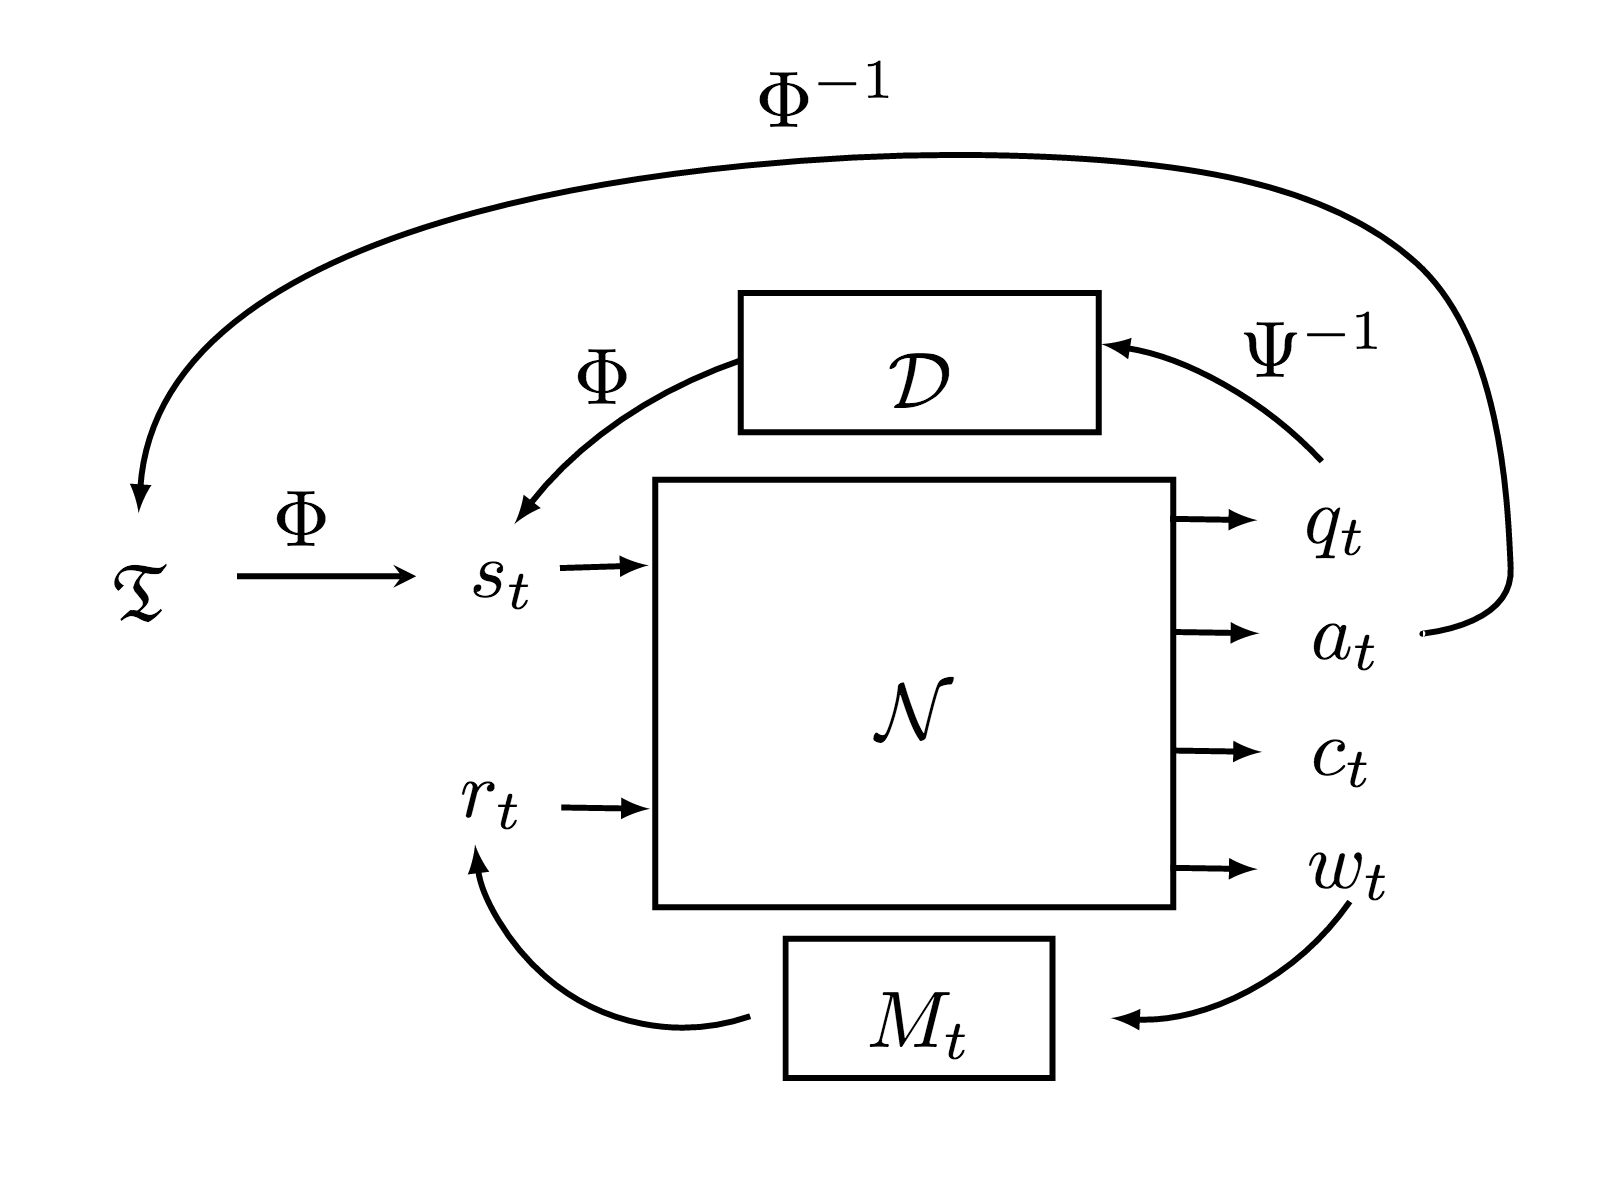
\includegraphics[width=\columnwidth]{jamesdiag}}
\caption{System architecture}
\label{sysarch}
\end{center}
\vskip -0.2in
\end{figure}
% \begin{figure*}
%     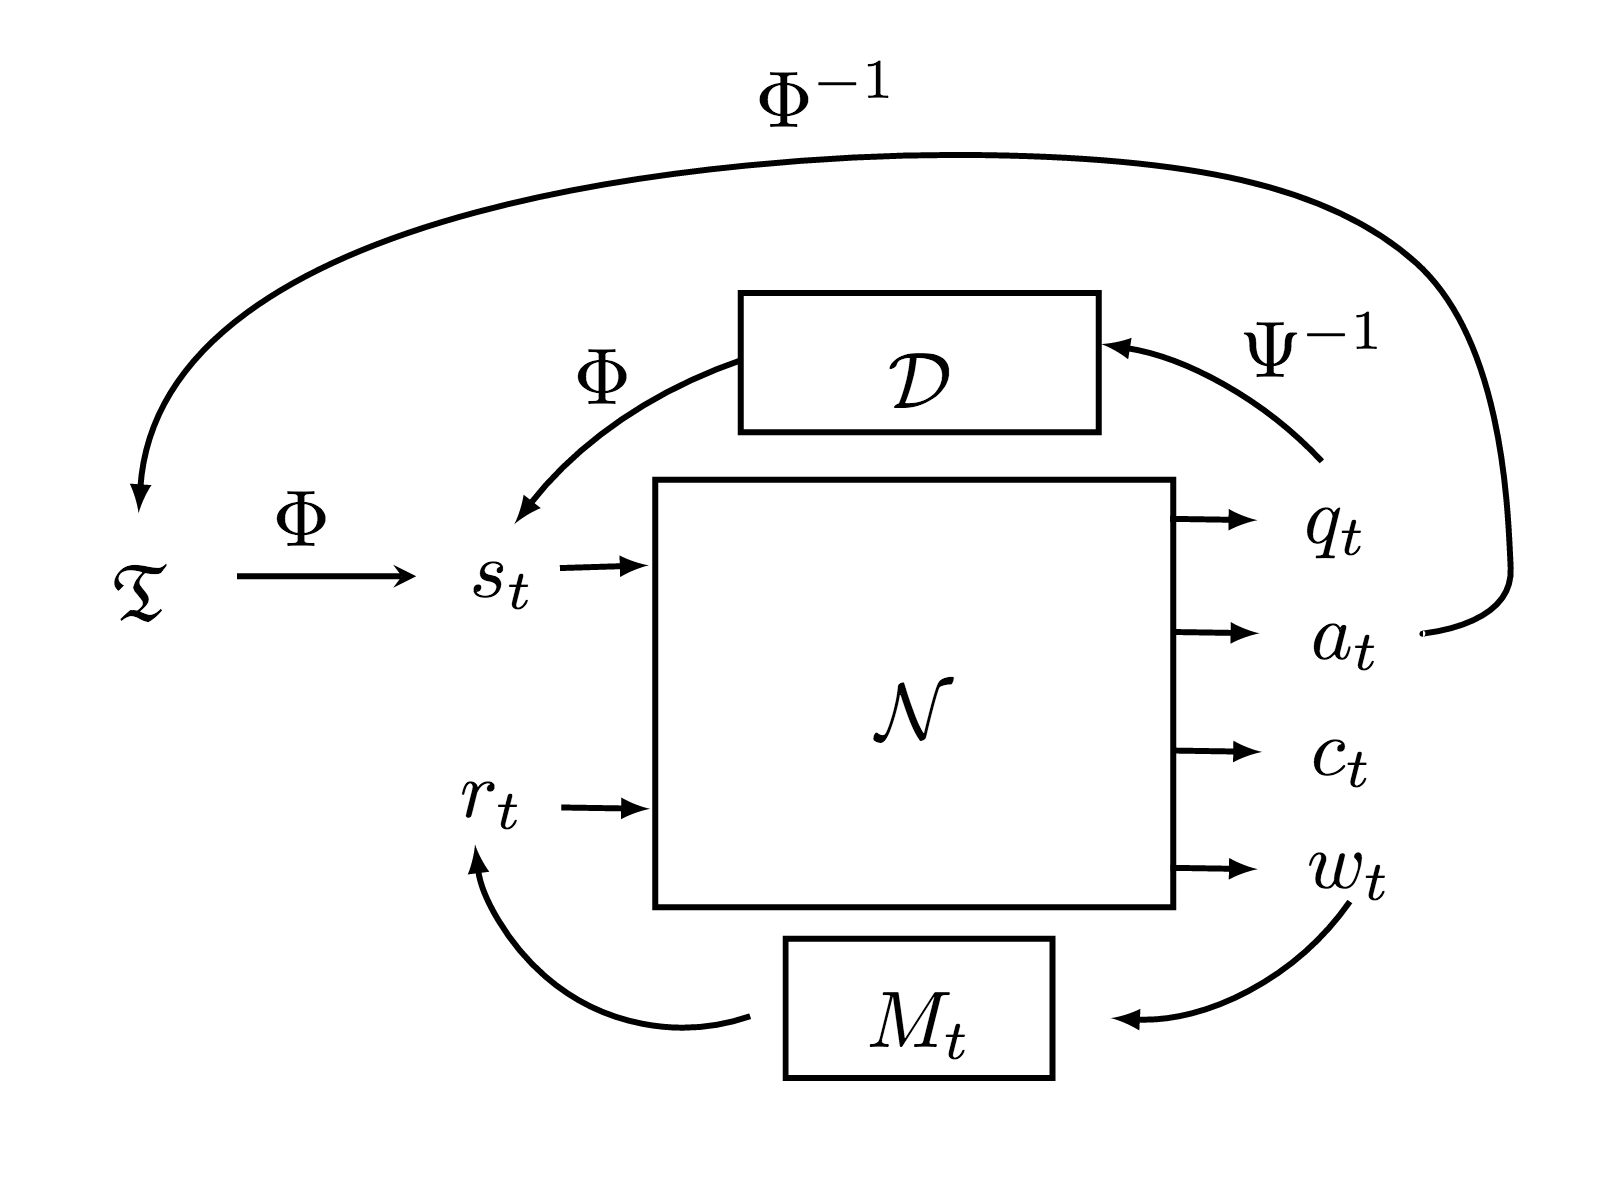
\includegraphics[scale=0.25]{jamesdiag}
%   \caption{System architecture}
% \end{figure*}
% \begin{figure*}
%     
\begin{tikzpicture}[scale=0.75]
\node[rectangle] at (0,0) (A) {$s_t$};
\node[rectangle] at (1.75,0) [draw,thick,minimum width=0.2cm,minimum height=1.8cm, fill=black] (BC1) {};
\node[rectangle] at (2.25,0) [draw,thick,minimum width=0.2cm,minimum height=1.8cm, fill=black] (BC2) {};
\node[rectangle] at (1.5,0) [draw,thick,minimum width=0.3cm,minimum height=2cm] (B1) {};
\node[rectangle] at (2,0) [draw,thick,minimum width=0.3cm,minimum height=2cm] (B2) {};
\node[rectangle] at (2.5,0) [draw,thick,minimum width=0.3cm,minimum height=2cm] (B3) {};
\node[rectangle] at (3.5,0) (action) {$a_t$};
\draw[->] (B3.east) edge (action.west);
\draw[brace] (B1.north) -- node [position label,yshift=2ex] {$\mu$} (B3.north);
\draw[->] (A) edge (B1);

\node[rectangle] at (2.7+ 1.75,-1.5) [draw,thick,minimum width=0.2cm,minimum height=1.8cm, fill=black] (QC1) {};
\node[rectangle] at (2.7+ 2.25,-1.5) [draw,thick,minimum width=0.2cm,minimum height=1.8cm, fill=black] (QC2) {};
\node[rectangle] at (2.7+ 1.5,-1.5) [draw,thick,minimum width=0.3cm,minimum height=2cm] (Q1) {};
\node[rectangle] at (2.7+ 2,-1.5) [draw,thick,minimum width=0.3cm,minimum height=2cm] (Q2) {};
\node[rectangle] at (2.7+ 2.5,-1.5) [draw,thick,minimum width=0.3cm,minimum height=2cm] (Q3) {};
\draw[brace] (Q1.north) -- node [position label,yshift=2ex] {$Q^\mu$} (Q3.north);
\draw[->, bend right] (A) edge (Q1.west);
\draw[->, bend right] (action) edge (Q1.west);
\node[rectangle] at (2.7+ 4,-1.5) (critic) {$Q^{\mu}(s_t, a_t)$};
\draw[->] (Q3.east) edge (critic.west);
\end{tikzpicture} 
%   \caption{DDPG architecture}
%   \end{figure*}

Formally, we model a conversation as an \emph{environment}, which is a Markov decision process, generally represented as a tuple $E=(\scripts, \scripta, \scriptr, T, r)$ where $\scripts$ is the statespace, $\scripta$ is the action space, $\scriptr$ is the reward space, and $T, r$ are the transition and reward functions respectively\footnote{For a high level overview of the MDP learnign set up, the reader is referred to \textbf{ TODO: insert reference}}. Given an environment, a (deterministic) agent is a map $\pi: \scripts \to \scripta$ which takes actions conditioned on state space. In the context of a \emph{conversational environment}, the state space is some featurized of the dialogue produced by the other party (the user) with whom Alexa communicates. Coorespondingly the action space is the dialogue that Alexa produces in response. As aforementioned, a conversationalist is rewarded under $r$ for maximizing engagement constrained to a minimal information theoretic throughput. Given the difficulty of defining such a function, we will learn $r$ based on actual conversation as depicted in Section 3; thus we suppose that $r$ is well defined.

Depicted in Figure \ref{sysarch} we seperate the approximation of an optimal policy $\pi$ into three components: dialogue representation, internal knowledge representation, as mentioned information lookup.
\begin{enumerate}
\item Dialogue representation is an embedding $\phi: \mathfrak{T} \to \scripts = \mathbb{R}^n$ from dialogue text into some suitable vector representation of semantics conditioned on context. Respecting that this task is still an active area of research, we will model $\phi$ and its inverse by experimenting with a variety different approaches such as thought vectors \cite{NIPS2015_5950}, sparse distributed representations of syntax trees \cite{DBLP:journals/corr/YogatamaFDS14}, and others (\textbf{HELP WITH ENGLISH)}.

\item Our requirement that $\pi$ activeley learn, manipulate, and act on an internal episodic knowledge representation of its current conversation, is analygous to the problem of one-shot learning. Therefore we approximate an optimal $\pi$ using a deep differentiable neural computer (DNC)\cite{graves2016hybrid}\cite{DBLP:journals/corr/GravesWD14} otherwise known as memory augmented network as motivated by the results of (\citeauthor{DBLP:journals/corr/SantoroBBWL16}, 2016).

In its simplest form the DNC is a map $\scriptn: (s_t, r_t) \mapsto (a_t, c_t, w_t)$ where  $r_t, w_t$ are the inputs and ouputs from \emph{read} and \emph{write} heads respectively. At every time step $\scriptn$ writes to an internal memory matrix $M_t$ at a specific address as specified by the controller output $c_t$. The DNN representation of $\scriptn$ will be implimented using a combination of FC and LSTM layers so as to provide $\pi$ with the ability to maintain an tempoorally conditioned representation of state. As per the training regime to be specified later, we will conditon the DNC to use the its memory augmentation to store an internal representation of facts learned during the course of a conversational episode in $E$.


\item Lastly, we describe a novel approach to external information lookup which is central to the social bot's ability to communicate details about popular topics. We define a set of documents $\scriptd \subset \mathfrak{T}$ and assume $\scriptd$ is \emph{locally} homeomorphic to some linear manifold $\Omega \subset \mathbb{R}^m$. Then let $\psi: \scriptd \to \Omega$ be that embedding. Finding such an embedding is a recent but promising development in NLP, with application to unsupervise search\cite{DBLP:journals/corr/DaiOL15}.

We wish to agument $\pi$ with the capability to request external information in a format compatible with its internal knowledge representation. Thus we add to $\scriptn$ a query output output $q_t \in \Omega.$ Procedurally we find the nearest document in $\Omega$, say $d_t$, and then use the text of the document as dialogue input into $\scriptn$ via $\phi$; that is,
\begin{equation*}
  \begin{tikzcd}
    & \scriptd \subset \mathfrak{T} \arrow{ld}[above]{\phi} & \\
    \scripts \arrow{rr}{\scriptn} & & \Omega \arrow{lu}[above]{\psi^{-1}}
  \end{tikzcd}
\end{equation*}
Requiring that $\pi$ only learn which class of documents are useful for responding in an engaging fashion is a much milder condition than assuming that $\scriptn$ will encode the details of every document in $\scriptd$. This novel approach to information lookup primes the memory of $\scriptn$, $M_t$ so that the details of a particular topic of discussion are at hand during a  episode, much in the same way that episodic conversational details are likewise written to $M_t$.
\end{enumerate}


\section{Training}
With the core architectural components of the model developed, we draw from a state of the art development in RL, inverse reinforcement learning\cite{ng2000algorithms}, to impart natural and expert level conversational skill on the Social Bot.

The principle idea behind inverse reinforcement learning is that behavioral cloning is limited to a biased distribution of only expert examples; that is, if the social bot’s model is trained to exactly replicate a human level conversationalist's response to different dialogues, then its ability to extrapolate beyond that known set of dialogues is unstable due to the severe nonlinearity of the model itself. In answer to this, inverse reinforcement learning attempts to infer the reward function of the agent being cloned. Knowing the reward function which an expert policy maximizes across a variety of states allows that policy to be cloned in a robust and dynamical fashion independent of the particular states in which it has acted; the cloned policy learns not about the particular examples to which it is tuned, but about the general principles which govern the expert policy.


In the context of the social bot, learning to communicate by understanding the forces which govern human level conversation as opposed to mimicking the conversation itself has immediate and fundamental benefits which have not yet been utilized in natural language processing. Therefore we propose the following training regime for our model.

To train parts $(1)$ and $(2)$ in our model, we take a variety of data sources containing conversation as described in the technical approach document (Public Conversation Corpus, News Interview Corpus, Late Night Show Corpus) \textbf{TODO desribe these datasets in the technical approach} and fix a conversationalist and an environment; that is, in all instances of conversation we specify a party $\hat{\pi}$ whose maximal reward function, $\hat{r}$ is to be learned, and a party who for all intents and purposes acts as $E$. Then with respect to the inversed party, we learn the action-value function $\hat{Q}: \scripts \times \scripta \to \scriptr$ which estimates the expected future reward of $\hat{\pi}$ recursiveley
\begin{equation*}
    \hat{Q}(s_t, a_t) = \expect_{s_{t+1} \sim E}\left[\hat{r}(s_{t}, a_t) + \gamma \hat{Q}(s_{t+1}, \mu(s_{t+1}))\right]
\end{equation*}
In addition to learning the action-value function, as perscribed in our technical approach, we learn a critic network $\epsilon: \scripts \times \scripta \to \mathbb[R}$ in the style of GANS \textbf{TODO write out this acronym} which estimates the engagement of the conversation as per the Mechanical Turk dataset. Accompanying $\epsilon$ is a prior on the density of engagement labels in state space, $P(\epsilon | s)$, which we use to derive the following update rule.

As per the standard deterministic policy gradient \textbf{TODO CITE SILVER 14 DPG } regime, assume that $\scriptn$ is parameterized by $\theta$ and then maximize the engagement and reward of a conversation by following the gradient
\begin{equation*}
	\theta' \leftarrow \theta + \left( \nabla_a \hat{Q}(s, a)  + P(\epsilon | s)\nabla_a \epsilon \right)\nabla_\theta  \scriptn.
\end{equation*}

Lastly, to train information retrieval we use the Washington Post News Interview dataset which contains conversations and cooresponding news articles (documents in $\scriptd$). Holding constant a proportion of the parameters of $\theta$, we define a conversation about a particular document to have an environment = the interviewer, agent the interviewee. \textbf{TODO SOMEONE FINISH THIS PIECE}. Then we take  $\hat{Q}$ learned from inverse reinforcement learning and apply it to
% We then take the conversation corpus
% Conversation Corpus
% News Interviews
% Articles and corresponding videos by news anchors
% Late Night Shows
% Engagement
% Label uniform sparse subset of some conversation data according to engagement, termination, depth
% Train a “critic”/adverserial  in the flavor DDPG or DCGAN
% Knowledge Retrieval
% News Interviews:
% Create another reinforcement learning regime where the actions are a document code, freezing the conversational portion of the network. Then perform a reverse lookup (using the nearest document in the embedded space) and feed that into the document read heads of the network.,
% Again reward the agent for correctly satisfying the reward function that was inverted from the conversations. From `(1.b)
% Conversation corpora


\printbibliography


\end{document}
